%%%%%%%%%%%%%%%%%%%%%%%%%%%%%%%%%%%%%%%%%%%%%%%%%%%%%%%%%%%%%%%%%%%%%%%%%%%%%%%%
\documentclass[a4paper, 10 pt, conference]{ieeeconf}
\usepackage{stylesheet}



%-----------------------------------------------------------
%-
%-  Titel
%-
%-----------------------------------------------------------
\title{\LARGE \bf Summary of ``Einführung in die Informationssicherheit''}

%-----------------------------------------------------------
%-
%-  Authors
%-
%-----------------------------------------------------------
\author{Martin Winter}

%%%%%%%%%%%%%%%%%%%%%%%%%%%%%%%%%%%%%%%%%%%%%%%%%%%%%%%%%%%%%%%%%%%%%%%%%%%%%%%%
\begin{document}

\maketitle
\thispagestyle{empty}
\pagestyle{empty}


%%%%%%%%%%%%%%%%%%%%%%%%%%%%%%%%%%%%%%%%%%%%%%%%%%%%%%%%%%%%%%%%%%%%%%%%%%%%%%%%
%-----------------------------------------------------------
%-
%-  abstract
%-
%-----------------------------------------------------------
\begin{abstract}

This document should serve as a summary of the necessary information given in the lecture ``Einführung in die Informationssicherheit''

\end{abstract}


%%%%%%%%%%%%%%%%%%%%%%%%%%%%%%%%%%%%%%%%%%%%%%%%%%%%%%%%%%%%%%%%%%%%%%%%%%%%%%%%

%-----------------------------------------------------------
%-
%-  Introduction
%-
%-----------------------------------------------------------
\section{ABBREVIATIONS and STANDARD NOTATION}
\begin{table}[h!]
    \begin{center}
    \begin{tabularx}{\columnwidth}{c c} % right-aligned, column separation by =-sign (and some whitespace to the left and to the right), left-aligned, centered, siunit: aligned at comma
        \toprule
       Abbreviation & Notation \\
        \midrule
        AES & Advanced Encryption Standard \\
        CBC & Cipher Block Chaining mode \\
        CFB & Cipher FeedBack mode\\
        CRL & Certificate Revocation List\\
        DES & Data Encryption Standard \\
        DHP & Diffie-Hellman problem \\
        DLP & Discrete logarithm problem \\
        DN & Distinguished Name \\
        DPA & Differential Power Analysis \\
        DSA & Digital Signature Algorithm \\
        ECB & Electronic Codebook mode \\
        ECDLP & Elliptic Curve Discrete Logarithm Problem \\
        ECDSA & Elliptic Curve Digital Signature Algorithm \\
        GDLP & Generlized discrete Logarithm Problem \\
        HW & Hamming Weight \\
        IDS & Intrusion Detection System \\
        IFP & Integer Factorization Problem \\
        LSB & Least Significant Bit \\
        MAC & Message Authentication Code \\
        MDC & Modification Detection Code \\
        MSB & Most Significant Bit \\
        OFB & Output Feedback mode \\
        OID & Object Identifier \\
        PGP & Pretty Good Privacy \\
        PKI & Public Key Infrastructure \\
        RSA & Rivest-Shamir-Adleman encryption scheme \\
        SCA & Side-Channel Attack \\
        SPA & Simple Power Analysis \\
        SSCA & Simple Side-Channel Attack \\
        DSCA & Differential Side-Channel Attack \\
        \bottomrule
    \end{tabularx}
    \end{center}
\end{table}

\pagebreak


%-----------------------------------------------------------
%-
%-  BASIC CRYPTOLOGIC PRINCIPLES
%-
%-----------------------------------------------------------

\section{\textbf{BASIC CRYPTOLOGIC PRINCIPLES}}
Because of the rise of digital communication, the value of information keeps growing, while it is subject to a large number of threats. 
This brings up the need to protect this information, hence Cryptography is the science of protecting information. 
A \textbf{cryptographic algorithm} is a \textbf{mathematical function}, that uses a \textbf{key} to encipher information, without this key, deciphering wouldn't be possible. 
\subsection{\textbf{CIA and Non-repudiation}}
Typically two entities want to \textbf{exchange messages securely} over an \textbf{insecure channel}, the \textbf{adversary} can now try to do several things, including eavesdropping the communication or altering it. 
\textbf{Eavesdropping} (Abhören) is a threat to the \textbf{confidentiality} of the message, a third member could possible read the content of the message. 
On the other hand, \textbf{altering} (Verändern) is a threat to the \textbf{integrity} of the message, therefore it is required to \textbf{authenticate} the communicating entities. 
The last of the security service deals is called \textbf{non-repudiation} (Nicht-Anerkennung), which means, that a sender cannot deny a message was sent, this property cannot be achieved by secret key cryptography alone unfortunately. 

\subsection{\textbf{Secret Key Cryptography}}
The most important requirement for such algorithms, besides their resistance against attacks, is that the reduction of performance is minimal. There are three types, which are discussed here
\begin{itemize}
\item \textbf{Block Ciphers} : Used to Encrypt Data
\item \textbf{Stream Ciphers} : Used as alternative
\item \textbf{MDCs}: Ensure integrity of data
\item \textbf{MACs}: For authentication
\end{itemize}

\vspace{0.5cm}

\subsubsection{\textbf{Block Ciphers}}
are defined as a set of boolean permutations on a \emph{n-bit} vector, this set contains a boolean permutation for each value of a key \emph{k}. 
It takes an element (from plaintext) and transforms it into an element from ciphertext.
Such a block cipher usually consists of several transformations, which form the encryption algorithm, those transformations happen several times, the transformation itself is called \emph{round function}, for each round a \emph{round key} $K_i$ is generated from the cipher key. 
There are mainly two different types of design, the \emph{Feistel ciphers} and the \emph{substitution permutation network (SPN)}. \\
There are also several modes of operation, whenever a message is longer than the block size, four modes are standardized. 
The \emph{electronic code book} (ECB) corresponds to the usual use case, the message is split into blocks and each block is encrypted separately with the same key. \\
In \emph{cipher block chaining} (CBC) each ciphertext block is x-ored with the next plaintext block before encryption. \\
In the \emph{output feedback} (OFB) mode and the \emph{cipher feedback} (CFB) mode, a keystream is generated and x-ored with the plaintext.

\subsubsection{\textbf{Stream Ciphers}} 
encrypt individual characters, usually bits, of a plaintext one at a time and use an encryption transformation, which varies with time. 
In contrast to block ciphers, this encryption not only depends on the key and plaintext, but also on the current state. \\
\textbf{Synchronous} stream ciphers generate a keystream independently of the plaintext, sender and receiver must therefore be synchronized (same key and same state within that key). \\
\textbf{Asynchronous} stream cipher is a stream cipher, in which the keystream is generated as a function of the key and a fixed number of previous ciphtertext bits. 
Because the keystream is dependent on only a few previous ciphertext bits, self-synchronization is possible even if some of the transmitted ciphertext bits are corrupted. 

\subsubsection{\textbf{MDCs}} 
take an input of arbitrary length and compress it to an output of fixed length, which is called the hash value. 
It satisfies the following properties
\begin{itemize}
\item \emph{preimage resistance}: computationally infeasible to find preimage to given hash value
\item \emph{2nd preimage resistance}: computationally infeasible to find 2nd preimage
\item \emph{collision resistance}: computationally infeasible to find two different inputs with same hash value
\end{itemize}
Hash functions are used to ensure the integrity of data, data is used as input to the hash function and the output is stored. It is possible to check the input for alteration by simply redoing the computation and comparing it with the original hash value. 

\subsubsection{\textbf{MACs}}
Hash functions, which involve a secret key, are called MACs (message authentication codes). The output of such a \emph{keyed hash function} is also called MAC, in contrast to MDCs they can also guarantee \textbf{data origin authentication} and \textbf{data integrity}. 
In order to ensure authenticity of data, an entity computes a MAC on the data using a private key, to verify the authenticity of the data later on, the MAC can be recomputed using the private key. 

\subsection{\textbf{Public Key Cryptography}}
In public key cryptography, secret keys are \textbf{replaced by keypairs}, consisting of a \textbf{private key}, which must be kept confidential, and a \textbf{public key}, which is openly accessible. \\
A message, encrypted by the public key, can be decrypted by the private key, this works, because the keys are linked in a mathematical way, such that knowing the public key does not allow to recover the private key, but enable independent encryption/decryption. 
\vspace{0.5cm}
\subsubsection{\textbf{RSA}}
\label{ex:rsa}
The Rivest-Shamir-Adleman(RSA) algorithm was the first public key encryption algorithm invented. It is based on IFP (Integer factorization problem) and keys are generated as follows: \\
One selects two large, \textbf{secret prime numbers} $p$ and $q$ and computes the public RSA modules
\begin{equation*}
n = p \cdot q
\end{equation*}
Then one chooses a public encryption exponent $e$ wich satisfies 
\begin{equation*}
gcd \left(e, (p-1)(q-1)\right) = 1 
\end{equation*}
gcd stands for \emph{greatest common divisor}. The private key $d$ can be calculated by solving
\begin{equation*}
e \cdot d = 1 \ mod \ (p-1)(q-1)
\end{equation*}
Hence the \textbf{public key} is the \textbf{pair (e,n)} and the \textbf{private key} is the \textbf{triple (d,p,q)}.\\
For encryption, the message needs to represented as a number $m < n$, the ciphtertext itself is computed by raising $m$ to the power of $e$
\begin{equation*}
c = m^{e} \ mod \ n
\end{equation*}
The message can be decrypted by exponentiation like
\begin{equation}
m  = c^{d} \ mod \ n
\end{equation}
\textbf{Example Key Generation}: \\
In real applications, p and q should at least be 512 bits!
\begin{align*}
p = 5 \quad q = 11 \\
n = p \cdot q = 55 \\
(p-1)(q-1) = 40 \\
\text{Random Number }e = 7 \\
gcd(e,(p-1)(q-1)) = 1 \\
d = e^{-1} \equiv 23 \ mod \ 40
\end{align*}
The public key is now $(e,n) = (7,55)$ and the private key is $(d,n) = (23,55)$. \\
\textbf{Example Encryption}: \\
\label{ex:rsa}
Encrypt the message M, assuming $M=25$ with public key $(e,n) = (7,55)$. 
\begin{equation*}
c = 25 ^{7} \equiv 20 \ mod \ n
\end{equation*}
\textbf{Example Decryption}: \\
Received message is $c = 20 \ mod \ 55$ and private key is $(d,n) = (23,55)$. This leads to 
\begin{equation*}
m = 20^{23} \equiv 25 \ mod \ 55
\end{equation*}

\vspace{0.5cm}
\subsubsection{\textbf{El Gamal}}

The El Gamal encryption algorithm is based on the DLP, and some public parameters can be shared by a group of users, called \emph{domain parameters}. This parameter is a \textbf{large prime p} (such that $p-1$ is divisible by another prime $q$) and an element $q \in \mathbb{Z}^{*}_{p}$ of order $p$ (or that the order is divisible by $q$. The \textbf{private key} $e$ can then be computed by solving
\begin{equation*}
e = g^{d} \ mod \ p
\end{equation*}

\textbf{Example Key Generation}: \\
In real applications, p should at least be 1024 bits!
\begin{align*}
p = 41 \quad g = 6 \quad d = 17 \\
e := g^{d} = 6^{17} \equiv 26 \ mod \ 41
\end{align*}
The private key $d$ is a random number between 2 and $p-1$. \\
\textbf{Example Encryption}: \\
Encrypt the message M, assuming $M=55$ with public key $(e,p,g) = (26,41,6)$. Then, use random number $k=11$ and compute 
\begin{align*}
c_1 = g^{k} = 6^{11} \equiv 28 \ mod \ 41 \\
c_2 = m\cdot e^{k} = 526^{11} \equiv 19 \ mod \ 41
\end{align*}
The encrypted message $(c_1,c_2) = (28,41)$ is now sent. 
\textbf{Example Decryption}: \\
Received message is $(c_1,c_2) = (28,41)$ and private key is $(d,p,g) = (17,41,6)$. This leads to 
\begin{equation*}
\frac{c_2}{c_1^{d}} = \frac{41}{28^{17}} \equiv 5 \ mod \ 41
\end{equation*}

\subsubsection{\textbf{ECC}}
ECC (Elliptic Curve)is a smooth curve in the so called \emph{Weierstrassform}. 
Similar to the El Gamal cryptosystem, several public parameters can be shared among a group of users.
These parameters are the elliptic curve group itself and the base point, the \textbf{private key} is a chosen integer $d$ and the public key is given by $e=dB$. 

\vspace{0.5cm}
\subsubsection{\textbf{Key Agreement}}
A major disadvantage of symmetric key cryptography is, that secret keys need to be distributed securely to the users. This problem can be solved using public key cryptography.


\vspace{0.5cm}
\subsubsection{\textbf{Digital Signatures}}
A digital signature is the equivalent of a handwritten signature, it binds someone's identity to a piece of information. A digital signature scheme consists of a \textbf{signature creation algorithm} and an associated \textbf{signature verification algorithm}. \\
Digital signatures \emph{with appendix} require the original message as input to the verification algorithm, digital signatures \emph{with message recovery} \textbf{do not} require the original message as input, it is recovered from the signature itself. 

The \textbf{DSS} is a standardized signatures scheme with appendix, which describes an algorithm called \textbf{DSA} (Digital Signature Algorithm) based on DLP, it has recently been extended and is now based on elliptic curves. \\
In order to sign a message, the owner first computes the hash value of the message, this value and the private key are then fed to the signing algorithm. 
The output is a signature of the input message, anyone who wishes to verify the signature can simply take the message, the public key and the signatures and compute the verification algorithm. 

\subsection{\textbf{Security and Attacks}} 
There exist many different types of attacks on cryptographic primitives, usually the goal is to deduce the secret key. \\
A \textbf{passive attack} is one, where the adversary only monitors the communication channel or the side-channels of the communication devices, they target the implementation, not the algorithm itself. \\
An \textbf{active attack} is one, where the adversary attempts to alter the transmission on the channel or the computation inside the device (\emph{fault attacks}). 
Side-channel attacks and fault attacks are so called \textbf{implementation attacks}, which pose a serious threat to cryptographic systems. 
To classify attacks, an assumption is made, that the adversary knows all details, except for the secret key. 
\begin{itemize}
\item \textbf{ciphertext-only}: deduce secret key by only observing ciphertext
\item \textbf{known-plaintext}: adversary has number of plaintext and corresponding ciphertexts
\item \textbf{chosen-plaintext}: adversary chooses plaintext and is given corresponding chiphertext
\item \textbf{adaptive chosen-plaintext}: choice of plaintext may depend on previous chipertexts
\item \textbf{chosen-ciphertext}: adversary chooses the ciphertext and is given the corresponding plaintext
\item \textbf{adaptive chosen-ciphertext}: choice of ciphertext may depend on previous plaintexts
\end{itemize}
Encryption schemes, which are vulnerable to ciphertext-only attacks, are considered completely insecure. 

\vspace{0.5cm}
\subsubsection{\textbf{Security Models}}
There are several different models, under which the security of a cryptograhpic primitive can be evaluated. 
\label{ex:secmod}
\begin{itemize}
\item \textbf{Unconditional security}: In this model, the adversary is assumed to have unlimited computational power, so this model is also called \emph{perfect secrecy}. A necessary condition is, that the secret key is at least as long as the message, because of that, systems like that are impractical. 
\item \textbf{Computational security}: Adversaries are assumed to have polynomial computational power, an algorithm is considered to be secure, if the best algorithm for breaking requires superpolynomial or exponential number of steps. 
\item \textbf{Provable security}: A cipher has provable security, if the difficulty of breaking can be shown to be equivalent to solving a well known, hard mathematical problem like DLP. 
\item \textbf{Practical security}: It is also related tot he computational power of the adversary, a cipher is considered practically secure, if the best \emph{known} attack requires at least $N$ operations, where $N$ is a sufficiently large number. 
\end{itemize}

\pagebreak 
\subsection{\textbf{Review Exercises}}

\subsubsection{\textbf{Name and explain the four security services (properties) cryptography can provide!}}
\begin{itemize}
\item confidentiality: "no unintended third party can understand the content"
\item integrity: "no one can change the message while it is in transit"
\item authentication: "get assurance of identity"
\item non-repudiation: "sender cannot deny a message was sent"
\end{itemize}

\subsubsection{\textbf{What is Kerckhoffs' principle?}}
The adversary knows all details about the used algorithms and protocols, only the secret key is unknown. 

\subsubsection{\textbf{What are the basic components of a block cipher?}}
The block cipher is a mathematical function, which takes plaintext as input, separates it into blocks, encrypts those with the secret key and has as output the ciphertext. 
Examples are DES (Data Encryption Standard) and AES (Advanced Encrpytion Standard). 

\subsubsection{\textbf{What is the difference between a block cipher and a stream cipher?}}
A block cipher encrypts blocks of data using a function dependent on the key, while a stream cipher generates a bitstream from the key and XORs it with the data. 

\subsubsection{\textbf{What is the difference between a MAC and an MDC?}}
MAC (Message Authentication Code)
\begin{itemize}
\item keyed hash-function (hash-value is signed)
\item ensures data integrity and data authentication
\end{itemize}
MDC (Modification Detection Code)
\begin{itemize}
\item unkeyed hash-function
\item ensure data integrity
\end{itemize}

\subsubsection{\textbf{What is the meaning of ``pre-image resistance''? For what cryptographic primitive is it relevant?}}
It should be computationally unfeasible, to find a pre-image to a given hash-value, this is relevant for MDCs (Modification Detection Codes). 
So it should be efficiently possible, to find the pre-image of a hash-value, meaning, finding a value that is mapped to a certain hash value. 

\subsubsection{\textbf{Explain how RSA encryption and decryption work!}}
Shown in (\ref{ex:rsa}). 

\subsubsection{\textbf{What is a digital signature with appendix?}}
A digital signature binds someones identity to a piece of information, those with appendix require the original message as input to the verification algorithm. 

\subsubsection{\textbf{Describe and explain the Diffie-Hellman Problem? What is it used for?}}
It is used for RSA, generally used for computing a common secret key. Two entities A and B agree to use a prime number $p$ and a base $g$, now A generates a secret random number $a$ and B $b$. Then A sends $g^{a} \ mod \ p$ and B sends $g^{b} \ mod \ p$ and both can compute $g^{ab} \ mod \ p$, which is their common secret key. 

\subsubsection{\textbf{Name and explain at least three different models of security}}
Shown in (\ref{ex:secmod}).

\subsubsection{\textbf{What does the term ``exhaustive key search'' mean?}}
All keys in the key space are being tried out, until the correct one is found. 




%-----------------------------------------------------------
%-
%-  ELECTRONIC SIGNATURES and PUBLIC KEY INFRASTRUCTURES
%-
%-----------------------------------------------------------
\section{\textbf{ELECTRONIC SIGNATURES and PUBLIC KEY INFRASTRUCTURES}}
\subsection{\textbf{Digital Signatures}}
A \textbf{digital signature} is a data string, which associates a message in digital form with some originating entity. \\
\textbf{DS with appendix} require the original message as input \\
\textbf{DS with message recovery} do not require the original message as input, the message is recovered from the signature itself.\\
\textbf{Randomized DS} has several valid signatures for a given message. \\
Most of the signatures schemes which are in use today, belong to the class of (randomized) digital signatures with appendix, this is due to the fact, that in most schemes, the hash of a message is signed instead of the message. 
This has advantages, the signatures are much shorter, when the hash is signed and several attacks, which apply for signatures schemes with message recovery can be thwarted (vereitelt) by signing the hash. Breaks can be classified as
\begin{itemize}
\item \textbf{Total break}: An adversary is either able to compute the private key or find an efficient signing algorithm, which is functionally equivalent to the valid signing algorithm
\item \textbf{Selective forgery}: An adversary is able to create a valid signature for a particular message or a class of messages a priori, creating the signature does not involve directly the legitimate signer.
\item \textbf{Existential forgery}: An adversary is able to forge a signature for at least one message, there is little or no control over the message and the legitimate user may be involved in the deception. 
\end{itemize}
Attacks can be classified to the capabilities of the attacker
\begin{itemize}
\item \textbf{Key-only attack}: Adversary knows signer's public key
\item \textbf{Known-message attacks}: Adversary has signatures for a set of messages, which are known to him.
\item \textbf{Chosen-message attacks}: Adversary obtains valid signatures from a set of messages, chosen by him. 
\item \textbf{Adaptive chosen-message attack}: Adversary may request signatures which depend on the signer's public key and he may request signatures, which depend on previously obtained signatures. 
\end{itemize}

\vspace{0.5cm}
\subsubsection{\textbf{RSA Signature Scheme}}
Key setup is the same as in RSA encryption, $m$ denotes the input message, $n$ the modulus, $d$ the private key and $e$ the public key.\\
\begin{table}[h!]
  \begin{center}
    \begin{tabularx}{\columnwidth}{ l   }
    \toprule
    \textbf{Algorithm 1} RSA Signature Creation \\ \midrule
    \textbf{Input:} $m,n,d$ \\ 
    \textbf{Output:} $Sig(m)$ \\
 1.) $M = Encode (m)$ \\
 2.) $s = M^{d} \ mod \ n$ \\
 3.) return $s$ \\

    \bottomrule
    \end{tabularx}
  \end{center}
\end{table}

\pagebreak
\begin{table}[h!]
  \begin{center}
    \begin{tabularx}{\columnwidth}{ l   }
    \toprule
    \textbf{Algorithm 2} RSA Verification Creation \\ \midrule
    \textbf{Input:} $m,s,e$ \\ 
    \textbf{Output:} Accept/Reject \\
    1.) Check length of $s$, if invalid then Return \emph{Reject} \\
    2.) $M = s^{e} \ mod \ n$ \\
    3.) If $M=Encode(m)$, then Return \emph{Accept}, else \emph{Reject} \\
    \bottomrule
    \end{tabularx}
  \end{center}
\end{table}


\vspace{0.5cm}
\subsubsection{\textbf{DSA Signature Standard (DSS)}}
It requires the usage of a hash function, originally SHA-1 was required, but now other hash functions are also allowed. \\
The numbers created by the key generations algorithm are the two primes $p$ and $q$, the element $\alpha$ with order $q$, the private key $x$ and the corresponding public key $y$.
\begin{table}[h!]
  \begin{center}
    \begin{tabularx}{\columnwidth}{ l   }
    \toprule
    \textbf{Algorithm 3} DSA Key Generation \\ \midrule
    \textbf{Input:}  \\ 
    \textbf{Output:} $p,q,\alpha,x,y,g$ \\
    1.) Choose prime $q$ such that $2^{N-1} < q < 2^{N}$ \\
    2.) Select another prime $p$ such that $2^{L-1} < q < 2^{L}$ and with the \\
    property that $q|(p-1)$ \\
    3.) Choose $\alpha$ of order $q$, it holds then that $\alpha = g^{(p-1)/q}$ \\
    4.) Choose a random integer $x$ such that $1 \leq x \leq q-1$ \\
    5.) Compute $y = a^{x} \ mod \ p$ \\
    6.) Return public key ($p,q,\alpha,y$) and private key $x$\\
    \bottomrule
    \end{tabularx}
  \end{center}
\end{table}

\begin{table}[h!]
  \begin{center}
    \begin{tabularx}{\columnwidth}{ l   }
    \toprule
    \textbf{Algorithm 4} DSA Signature Creation \\ \midrule
    \textbf{Input:} $m,x$ \\ 
    \textbf{Output:} Sig(m) \\
    1.) Choose a random $k$, $0 < k < q$ \\
    2.) Compute $r = (a^k \ mod \ p) \ mod \ q$ \\
    3.) Compute $s = k^{-1}(h(m) + xr) \ mod \ q$ \\
    4.) Return the signature for $m$ which is $(r,s)$\\
    \bottomrule
    \end{tabularx}
  \end{center}
\end{table}

\begin{table}[h!]
  \begin{center}
    \begin{tabularx}{\columnwidth}{ l   }
    \toprule
    \textbf{Algorithm 5} DSA Signature Verification \\ \midrule
    \textbf{Input:} $m,(r,x),y$ \\ 
    \textbf{Output:} Accept/Reject \\
    1.) Verify that $0 < r < q$ and $0 < s < q$\\
    2.) Compute $u_1 = wh(m) \ mod \ q$ and $u_2 = rw \ mod \ q$ with \\ $w = s^{-1} \ mod \ q$ \\
    3.) Compute $v = (\alpha^{u_1}y^{u_2} \ mod \ p) \ mod \ q$ \\
    4.) Return the signature for $m$ which is $(r,s)$\\
    5.) Return \emph{Accept}, if $v=r$, otherwise return \emph{Reject}. \\
    \bottomrule
    \end{tabularx}
  \end{center}
\end{table}


\vspace{0.5cm}
\subsubsection{\textbf{ECDSA Signature Scheme}}
The elliptic curve digital signature algorithm (ECDSA) is the analogue to the DSA, the major difference is, that the DLP, which gives the algorithm its security, is hereby defined over an elliptic curve. 
Two entities choose a finite field $\mathbb{F}_q$, an elliptic curve E, defined over that field and a base point G with order n. One key pair is $(d,Q)$, where $d$ is her private and $Q$ is her public key. 

\begin{table}[h!]
  \begin{center}
    \begin{tabularx}{\columnwidth}{ l   }
    \toprule
    \textbf{Algorithm 6} ECDSA Signature Creation \\ \midrule
    \textbf{Input:} $m,d$, elliptic curve with base point $G$ of order $n$ \\ 
    \textbf{Output:} Accept/Reject \\
    1.) Chosse a random number $k$ with $k: 1 \leq k \leq n-1$\\
    2.) Compute $kG = (x_1,y_1)$ and $r = x_1 \ mod \ n$. If $r=0$,\\ then go to step 1. \\
    3.) Compute $k^{-1} \ mod \ n$ \\
    4.) $e = h(M)$ \\
    5.) Compute $s = k^{-1}(e+dr) \ mod \ n$. If $s=0$, then go to step 1. \\
    6.) Return the signature which is $(r,s)$ \\
    \bottomrule
    \end{tabularx}
  \end{center}
\end{table}
\begin{table}[h!]
  \begin{center}
    \begin{tabularx}{\columnwidth}{ l   }
    \toprule
    \textbf{Algorithm 7} ECDSA Signature Verification \\ \midrule
    \textbf{Input:} $m,(r,s),Q$, elliptic curve \\ 
    \textbf{Output:} Accept/Reject \\
    1.) Verifiy, that $r,s$ are integers in the intervall $[1,n-1]$ \\
    2.) compute $e = h(M)$ \\
    3.) Compute $w = s^{-1} \ mod \ n$ \\
    4.) Compute $u_1 = ew \ mod \ n $ and $u_2 = rw \ mod \ n$ \\
    5.) Compute $X = u_1G + u_2G$ \\
    6.) \textbf{if} $X=0$ \textbf{then} \\
    7.) 	  Return Reject \\
    8.) \textbf{else} \\
    9.) Compute $v=x_1 \ mod \ n$ where $X=(x_1,y_1)$ \\
    10.) Return Accept if $v=r$, else return Reject!\\
    \bottomrule
    \end{tabularx}
  \end{center}
\end{table}


\subsection{\textbf{Public Key Infrastructures}}
Even public keys need protection, because adversaries could try to modify published public keys. 
So there needs to be some mechanism to check their authenticity, meaning to check, if a certain key belongs indeed to a certain person. 
A public key infrastructure (PKI) is the basis of a security infrastructure, whose services are implemented and delivered by using public-key concepts and techniques. 
\vspace{0.5cm}
\subsubsection{\textbf{Public Key Distribution}}
Different possibilities for distributing public keys include the \emph{face-to-face approach}, isn't practical, the person would need to meet with everyone who wishes to obtain her public key in person. \\
The second option is, that the person publishes her key on a trusted web server and anyone, who wishes to obtain the key simply looks there. Is still impractical, because there is no way to verify the identity and integrity of the key. \\
The third option is, that the certified public key is stored on a trusted web server, meaning that the trusted web server provides a service, which adds additional information to a key, the so-called \textbf{certificate}.
A certificate basically consists of a public key and some user information, which has been digitally signed by the issuer of the certificate. 
\vspace{0.5cm}
\subsubsection{\textbf{PGP}}
In a PGP based PKI, each user acts a s a third party, who can sign keys. Each user also manages keys herself, hence, there is no need for a central controlling authority, it is based on the so-called \textbf{user-centric trust model}. Each user trusts herself and a limited amount of other users. 
For example, Alice trusts Bob, hence she trusts all the keys, which have been signed by Bob, so if Bob trusts Clark, then also Alice trusts Clark. \\
The problem here is, that it is implicitly assumed, that \textbf{trust is transitive}, also the \textbf{revocation} (Widerruf) is difficult. 
\vspace{0.5cm}
\subsubsection{\textbf{X.509}}
The trust model, which is the basis for X.509-based PKIs is the hierarchical trust model, there exists a so-called \textbf{root CA}, which acts as root or anchor of trust for the entire domain of entities below it, it owns a root-certificate, which is the basis of trust for all entities, that belong to the domain. The root CA certifies CAs immediately below it, who certify again some CAs below them and so on. \\
At the second to last level, the CAs certify end entities. \textbf{Each entity in the hierarchy} must be \textbf{supplied with the certificate of the root CA}. \\
The advantage is, that because of the hierarchical structure, revocation checking can be reliably implemented, disadvantages are, that they tend to be big and complex.

\vspace{0.5cm}
\subsubsection{\textbf{X.509 Certificates}}
A certificate is a data structure, which essentially \textbf{consists of the public key} of an entity \textbf{plus some information about the entity}, and it is \textbf{digitally signed} by the certificate issuer. 
\begin{figure}[h!]
\centering
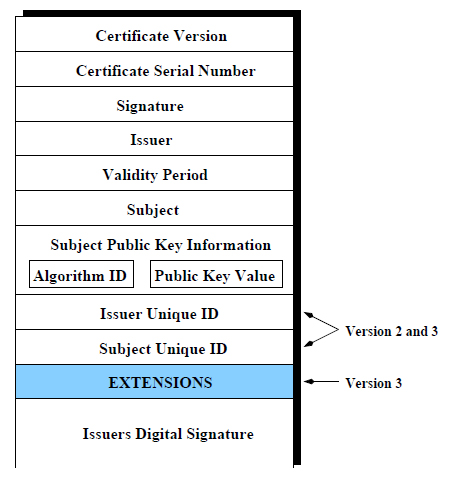
\includegraphics[scale=0.44]{images/diagrams/x509.jpg} 
\end{figure}

\pagebreak

An \textbf{OID} is a unique representation for a given object, for example an algorithm or a standard, it is represented as a sequence of integers separated by decimal points. They are hierarchical and they are registered with authorities to ensure uniqueness. \\
A \textbf{DN} is a hierarchical naming convention, they are supposed to ensure the unique name of an entity and are expressed as a concatenation of relative DNs from toe top-level node down to the last node of DN. 

\subsubsection{\textbf{X.509 PKI Components}}
\begin{itemize}
\item \textbf{Registration Authority (RA)}: Often, a separate registration authority is used to verify the identity of entities. For highly trusted certificates, the verification of the identity requires physical presence of the entity.
\item \textbf{Certification Authority (CA)}: The certification authority issues certificates to entities, which have already been identified. 
\item \textbf{Certificate Repository}: The certificates are stored in the certificate repository, those can be implemted using LDAP (lightweight directory access protocol).
\item \textbf{Certificate Revocation}: The revocation of issued certificates is hardly implemented in practice, instead, most mechanisms are focused on the distribution of revocation information. 
\end{itemize}


\vspace{0.5cm}
\subsection{\textbf{Legal Aspects of Electronic Signatures}}
The legal definition of an electronic signature is given as follows
\begin{center}
\textit{Data in electronic form, which are attached to or logically associated with other electronic data and which serve as a method of authentication.}
\end{center}
According to the above mentioned directive, the validity of this electronic signature cannot be denied solely based on the fact, that it is in electronic form. 

\subsubsection{\textbf{Advanced Electronic Signatures}}
\label{sig:adv}
An \emph{advanced electronic signature} must be uniquely linked to the signatory (Unterzeichner). It also must be capable of identifying the signatory and must be created using means, that the signatory can maintain under his sole control. It also must be linked to the data, to which it relates, in such a manner, that any subsequent change of the data is detectable. \\
This type of electronic signatures are not considered equal to handwritten signatures from a legal point of view. 

\subsubsection{\textbf{Qualified (Secure) Electronic Signatures}}
A \emph{qualified (secure) electronic signature} is an advanced electronic signature, which was produced on a secure signature creation device and which is based on a qualified certificate. It must be assured, that the signature creation data (private key) exists only once and is protected by the user. \\
The Austrian Signature Law (SigG) specifies that, apart from a few exceptions, a qualified digital signature is legally equivalent to a handwritten signature. 


\pagebreak
\subsection{\textbf{Electronic Signatures in Practice}}
Applications, that profit from electronic signatures, are primarily available in the e-government sector. 
The Austrian initiative is known as the concept "Bürgerkarte", in this concept, the so-called "Bürgerkartenumgebung" is the combination of the security-relevant components with respect to electronic signatures, applications communicate with the Bürgerkartenumgebung over the so-called \textbf{security layer}, which is an interface, that provides a logical view. 



\subsection{\textbf{Review Exercises}}
\subsubsection{\textbf{What is a digital signature?}}
In the language of cryptographers, a \emph{digital signature} is a data string, which associates a message in digital form with some originating entity. 
\subsubsection{\textbf{What classes of digital signatures can you distinguish?}}
\begin{itemize}
\item DS with appendix
\item DS with message recovery
\item Randomized DS
\end{itemize}
\subsubsection{\textbf{What types of breaks of digital signatures schemes can you distinguish?}}
\begin{itemize}
\item \textbf{Total break}: An adversary is either able to compute the private key or find an efficient signing algorithm, which is functionally equivalent to the valid signing algorithm
\item \textbf{Selective forgery}: An adversary is able to create a valid signature for a particular message or a class of messages a priori, creating the signature does not involve directly the legitimate signer.
\item \textbf{Existential forgery}: An adversary is able to forge a signature for at least one message, there is little or no control over the message and the legitimate user may be involved in the deception. 
\end{itemize}
\subsubsection{\textbf{Describe the working principle of a digital signature scheme with appendix!}} 
Signatures with appendix require the message as input for the verification.
\subsubsection{\textbf{What is a PKI used for?}} 
PKI stands for Public Key Infrastructure, when using asymmetric encryption, the public keys have to be exchanged which can happen over a trusted web server. Besides the key there is also a certificate available, that guaranties, that the key hasn't been altered. 
\subsubsection{\textbf{What is the difference between a PGP-based and a X.509-based PKI?}} 
Difference lies in the trust modell.\\
\textbf{PGP}: Each user acts as CA and signs keys from other users, a user centric trust, if A trusts B and B trusts C, A also trusts C. \\
\textbf{X.509}: Hierarchical structure, root CA creates root certificate, can define some CAs below him, which also can certify CAs below them and so on, the second to last defines the end user. 
\subsubsection{\textbf{What is a CRL?}} 
A CRL (Certificate Revocation List) is a list of certificates, that have been revoked (für ungültig erklärt worden). 

\pagebreak
\subsubsection{\textbf{What is an advanced electronic signature?}} 
\begin{itemize}
\item It must be uniquely linked to the signatory
\item It must be capable of identifying the signatory
\item It must be created using means, that the signatory can maintain under his sole control
\item It must be lined to the data, which it relates to, in such a manner, that any subsequent change of the data is detectable. 
\end{itemize}
\subsubsection{\textbf{What type of electronic signature is equivalent (from a legal point of view) to a handwritten signature?}} 
Qualified electronic signatures are equivalent to handwritten signatures.
\begin{itemize}
\item advanced electronic signatures based on
\item secure signature-producing-process and based on qualified certificate
\item mandatory requirements like a private key must only exist once
\item the requirements are protected from harmful access of others
\end{itemize}

\raggedbottom

\pagebreak
\section{\textbf{ELECTRONIC COMMERCE}}
Electronic commerce, is the business of buying and selling products, information or services electronically, those are mostly conducted using a credit or debit card. 
Typically, e-commerce merchants store cardholder information in databases to streamline the process, hence, containing thousands of payment card accounts. 

\subsection{\textbf{E-shopping}}
E-shopping is a \emph{multi-phase process}. In the first phase, the customer browses through products, selected goods are typically put into a shopping cart and at the end of this process, the customer is usually asked to proceed to check out. 
In the second phase, the customer selects the payment and delivery options and in the third phase the goods are delivered. \\
One of the most important factors for the success of e-business is having a secure and reliable system, this depends on who's asking the question. 

\subsection{\textbf{Types of Payment}}
\textbf{Cash} is a floating claim on a bank or other financial institution, that is not linked to any particular account, it is a \emph{direct payment method}, it is well suited for occasional purchasing and for buying physical products but less suited for buying services, that are occur repeatedly. \\
Other types of payment systems are \textbf{checks} and \textbf{bank cards}. Checks are suitable for not to small payments, a disadvantage is the costly rejection of a check. \\
Bank cards are also suitable for any not too small value, the payee can be remote from the payer, many of those systems require only connections for verification nowadays. \\
\textbf{Credit systems} work differently, the customer has to register with a bank, if goods are purchased, they get debited on his account and the customer is only billded after a certain amount of time has passed or only once a month. \\
In a \textbf{debit system}, the customer pays before the purchase, such systems are suitable for subscriptions or any regular purchases. 

\subsection{\textbf{E-payments}}
\subsubsection{\textbf{E-money}}
\emph{E-money} or \textbf{digital currency} is simply an encoded string of digits and essentially consists of a serial number and the amount. 
It is a floating claim on a bank or other financial institution, that is not linked to any particular account. Expected Advantages are, that it is anonymous, and involved entities do not have to trust each other, and there follows the direct disadvantage, following the anonymity aspect, it is \textbf{not traceable}. \\
It is possible to distinguish \textbf{micropayments} and \textbf{macropayments}. \\
\textbf{Micropayments} are tiny value transactions below \$1, they are supposed to be cheap and a little cheating can be tolerated because of the minuscule amount. \\
\textbf{Macropayments} are medium value transactions (between \$1 and \$1000) and large value transactions (over \$1000). 
\label{tex:sect}
\begin{itemize}
\item \textbf{Security}: It is mandatory to prevent forgery, double spending and collusion of other parties (multi-party security)
\item \textbf{Acceptability}: A wide range of parties needs to accept the payments
\item \textbf{Convenience}: Factors that increase the convenience are speed, reliability, divisibility and transferability.
\item \textbf{Cost}: Virtually no cost should arise while dealing with digital currency, as it is with physical currency. 
\item \textbf{Privacy}: Cash is the most anonymous payment form, e-money should be as well. 
\item \textbf{Durability}: E-money shouldn't be easily lost, like during a system crash
\item \textbf{Independence}: E-money should be easily storable on different devices
\item \textbf{Transferability}: Cash can be easily exchanged between entities, should be the same for e-money.
\item \textbf{Divisibility}: Customer gets return money, if price is lower than the given amount in the physical world, should be the same for e-money.
\item \textbf{Immediate Control}: In case of a security breach, such as forgery of money, it must be possible to identify the security breach immediately. 
\item \textbf{Traceability}: Especially with large transactions, anonymous money can be a problem, some sort of tracing mechanism would be an advantage.
\item \textbf{Spread of Encryption Mechanisms}: E-money systems, which involve encryption heavily, might be difficult to export to other countries. 
\end{itemize}
Trade-offs include \label{tex:tradeoff}
\begin{itemize}
\item \textbf{Privacy vs Traceability}: Tiny value payments deserve to be anonymous, while for large value payments traceability is probably favourable. 
\item \textbf{On-line vs Off-line}: On-line payments allow to prevent double spending easily and simplify tracing transactions. Offline payments often use special purpose hardware to prevent double spending.
\item \textbf{Hardware vs Software}: Hardware solutions can also prevent double spending, but often hardware decrease the customer acceptance. 
\item \textbf{Transparency vs Explicitness}: User want to have control over all their transactions but they also expect not to be bothered with any details. 
\end{itemize}
\vspace{0.5cm}
Discussed will be the famous DigiCash system, coins there are anonymous, so the bank doesn't know, which coin belongs to which customer. Despite the anonymity, the system prevents multiple spending of coins, it allows even to determine with a high probability, who tried to double-spend money in case such a fraud occurred. 
\pagebreak
The protocol, describing the DigiCash system works as follows:
\begin{itemize}
\item \textbf{Money Generation Phase}:\\ Customer produces $n$ money orders with $n$ serial numbers and $n$ identity strings, then the customer "blinds" the money orders, so the bank doesn't see the serial numbers, so it is anonymous. The bank now checks $n-1$ money orders for their consistency, if valid, it signs the last remaining blinded money order with its private key, without seeing what's inside, customer now possesses an anonymous coin signed by the bank.
\item \textbf{Money Spending Phase}: \\
Merchant check the validity of the coin by checking bank signature. Then requests halves of the identity strings, randomly either the left or right one of each identity string and stores them.
\item \textbf{Double-spending Checking Phase}: \\
When merchant now deposits coin at the bank, signature is once again validated and the database is checked for the serial number. If the string is already present, bank checks stored identity strings, if merchant wanted to collect money twice, those strings will match. Otherwise there will be a pair of identity string halves, that will produce a full identity string and reveal the cheating customer. 
\end{itemize}


\vspace{0.5cm}
\subsubsection{\textbf{Bank cards}}
Bank cards nowadays are often smart cards and offer two different functionalities: Maestro and Quick. Whenever money is being put on a Quick Card, the PIN must be entered and is checked by an online system, those transactions are authorized by this central system. 
In all Quick terminals, there is a smart card which is used for "offline" payments. This card communicates with the customer card, saves information about the turnover and can provide additional authentication mechanisms. 
\vspace{0.5cm}
\subsubsection{\textbf{SET and its Successors}}
SET stands for \textbf{Secure Electronic Transactions} and is a specification for authentication for paying with credit cards within online networks, jointly developed by VISA and MasterCard. \\
In SET, the cardholder uses a software called an electronic wallet, in which the credit card numbers and digital certificate are stored. The merchant acquires a digital certificate from a financial institution and both cardholder and merchant use their certificates for authentication before a transaction. 
During a SET transaction, the credit card number is not seen by the merchant, only the encrypted number is sent to the credit card issuer, which approves the transaction for the merchant. In this way, disclosure is prohibited during the transaction. \\
The cryptographic means to ensure the privacy of customer data, it is called \textbf{dual-signature}, it allows the cardholder to communicate with both the merchant and the bank with one single message, which contains an order section plus a payment section
\begin{itemize}
\item The merchant does not need to see the payment section.
\item The bank does not need to see the order section. 
\item But, both sections need to be bound together. 
\end{itemize}
The disadvantage of SET were the significant investment required for cardholder, merchant and bank, in the mean time SET was replaced by proprietary systems from VISA (3d-Secure) and MasterCard(Master Card SecureCode). 

\subsection{\textbf{Alternative E-payment Methods}}
\begin{itemize}
\item PayPal
\item PaySafe Card
\item First Gate Click\& Buy
\item Google Wallet and NFC
\end{itemize}
More information about those payment options in script starting on page 41.


\subsection{\textbf{Review Exercises}}

\subsubsection{\textbf{What types of payment systems can you distinguish?}}
\begin{itemize}
\item Cash
\item Credit systems
\item Debit systems
\end{itemize}

\subsubsection{\textbf{What is the difference between micropayments and macropayments?}}
Micropayments describe payments below 1\$ and macro payments usually payments between 1\$ and 1000\$. 
\subsubsection{\textbf{Discuss 4 aspects of digital currency!}}
Shown in (\ref{tex:sect}).
\subsubsection{\textbf{Discuss the trade-offs that are typically made in electronic payment systems!}}
Shown in (\ref{tex:tradeoff}).
\subsubsection{\textbf{Explain in short, how money is generated in the DigiCash system!}}
Answer is on the left side! :) Money Generation Phase of DigiCash. 
\subsubsection{\textbf{What does SET mean and what was/is the SET system used for?}}
SET stands for Secure Electronic Transaction and is a specification for paying with credit cards, used in the past by VISA and MasterCard.
\subsubsection{\textbf{Explain the purpose of the dual signature in the SET system!}}
It allows the cardholder a sensitive way to pay, without the merchant seeing the payment details and without the bank seeing the order details, each part is encrypted using either the public key of the merchant or the bank, but both are bound together. 


\pagebreak







\section{\textbf{NETWORK SECURITY}}

Network security addresses all security issues, which come into play when two parties attempt to communicate over a network, which is typically not secure and trusted. This part focuses on attacks and counter-measures, which are not prevented by cryptographic methods. 

\subsection{\textbf{Social Engineering}}
Humans are always the weakest link in every security infrastructure and social engineering attacks target humans. In such attacks, the attacker tries to persuade a person to give access to his information. 
Problematic is, that even the best firewall and the best intrusion detection system will not defend you against an attacker, who got a password from one of the users. 
Social Engineering typically tries to achieve one of the following goals
\begin{itemize}
\item Physical access
\item Remote access credentials
\item Confidential information
\item Violation of other security controls
\end{itemize}

Social engineering attacks are further subdivided into \emph{active } and \emph{passive} attacks, in active attacks, the attacker actively interacts with the attacked person, in passive attacks the attacker acquires information with stealth.
\subsection{\textbf{OS Fingerprinting}}
\emph{OS fingerprinting} is a technique, in which the attacker tries to determine the operating system, which is running on the target machine. As much vulnerabilities, which can be exploited in an attack, are OS dependent, OS fingerprinting is typically the first step in a network attack. 
\vspace{0.5cm}
\subsubsection{\textbf{Telnet}}
\emph{Telnet session negotiation} is probably the simplest way to determine the OS, you simply have to open a telnet session to the remote server, those servers often respond with a whole bunch of information about the OS. 
\vspace{0.5cm}
\subsubsection{\textbf{TCP Stack Fingerprinting}}
Another way of gathering information about the OS running on a remote host is to look at how the TCP stack is implemented by the OS, in some operating systems, in particular Windows, the have very distinct implementations of the TCP stack, so the version can be identifies by sending special TCP packets and see, how the server reacts. Even without dedicated countermeasures, some obstacles can make fingerprinting difficult in practice, a packet can be modified while in transit, also filtering devices may change one or several field values of a packet. 



\subsection{\textbf{Attacking Internet Protocols}}

\subsubsection{\textbf{SYN Flooding}}
In a \emph{SYN flooding} attack, the adversary sends a large number of SYN packets (the first message in the TCP handshake protocol) to the remote hose and never acknowledge any of the replies, this way, the remote host accumulates more SYN packages than it can handle and this is a typical DoS (Denial-of-service) attack. \\
A technical solution is to use the SYNcookie and don't keep a copy of the incoming SYN packet, but hashed version of it, so sessions do not need to be kept half-open.
\vspace{0.5cm}
\subsubsection{\textbf{Smurfing}}
\label{smurf}
In a \emph{smurfing} attack, a vulnerability of the ICMP (Internet Control Message Protocol) is exploited, a user can send an echo packet to a remote host in order to check, if the host is alive. In a smurfing attack, the adversary constructs a packet with the source address forged to be that of the attacked computer and to send it to a number of other hosts.
The other hosts will respond by sending a packet to the target, if enough hosts respond, the target computer will receive more packets, than it can handle. 
\vspace{0.5cm}
\subsubsection{\textbf{DDoS Attacks}}
In \emph{distributed denial-of-service} (DDoS) attacks, an adversary takes over a large number of machines and installs custom attack software on them, at a pre-determined time or on a signal, the software activates and starts bombarding the target machine with messages. 
\vspace{0.5cm}
\subsubsection{\textbf{Spoofing}}
\emph{Spoofing} attacks combine some of the ideas, which are used in the previously described attacks, an adversary can use a DoS attack to take a web server, the adversary now can attempt to initiate a connection to a user and can send messages in persona of the web server. The response of the user will be, however, directly to the web server. \\
The best way to detect a spoofing attack is to monitor the replay to the SYN+ACK packet, if the host is still alive, it will return a NACK, which can be used to identify this type of attack. 

\subsection{\textbf{Trojans, Viruses, Worms and other malicious code}}
A trojan, virus or a worm is essentially a piece of malicious code or software, roughly spoken, a \textbf{Trojan} is a program doing something malicious such as stealing passwords, a \textbf{worm} is a program, that replicates and a \textbf{virus} is a worm, that replicates by attaching itself to other programs. 


\vspace{0.5cm}
\subsubsection{\textbf{Taxonomy of Malicious Programs}}
Malicious programs can be divided into two categories, those that need a host program and those, who don't. In the first category fall \emph{trap doors, logic bombs, Trojan horses} and \emph{viruses}. 
In the second category fall \emph{worms} and \emph{zombies}. 
\vspace{0.5cm}
\subsubsection{\textbf{Trap doors}}
\label{trapd}
A trap door is a secret entry point into a program, this technique has been used legitimately for many years by programmers to debug and test programs. Such a trap door can be a part of the code that recognizes some special sequence for example. 
\vspace{0.5cm}
\subsubsection{\textbf{Logic Bombs}}
A logic bomb is some code in a program that is set to detonate, when certain conditions are met. Examples of such conditions are the presence or absence of certain files, date or a particular user. Once activated, a logic bomb may cause a machine halt, delete files or other stuff.
\vspace{0.5cm} 
\subsubsection{\textbf{Zombies}}
A zombie is a program, that takes over a computer, which is attached to the internet, to launch attacks that are difficult to trace to the creator of the zombie, they are often used in DDoS attacks. 
\vspace{0.5cm}
\subsubsection{\textbf{Viruses and Worms}}
A virus is a program, that infects other programs by modifying them. A virus or worm typically consist of two components, a \textbf{replications mechanism} and a \textbf{payload}. A simple replication mechanism is for example, when a worm makes a copy of itself wherever it runs. A trigger activates the payload. \\
Viruses and worms typically go through 4 phases during their lifetime
\label{virusphase}
\begin{itemize}
\item \textbf{dormant phase}: virus is idle
\item \textbf{propagation phase}: the virus infects other programs
\item \textbf{triggering phase}: virus is activated
\item \textbf{execution phase}: virus performs its function
\end{itemize}
\label{viruses}
There are \textbf{parasitic viruses} (attach themselves to executables and replicate), \textbf{Memory-resident viruses} (reside in main memory, infect every program, that executes), \textbf{Boot sector viruses} (infect MBR), \textbf{Stealth viruses} (hide from detection) and \textbf{Polymorphic viruses} (mutate with every infection). \\
There are different types of worms as well, in \textbf{Email}, \textbf{Remote Exectuion} (worms execute a copy of themselves on another system) and \textbf{Remote Login} (worms log onto remote systems as user and copy themselves from one system to the other). \\
\textbf{Countermeasures} against viruses and worms consist mainly of using antivirus software, that investigates programs for known strings of viruses. Another possibility is to keep a checksum of the original executable and check, if it changed over time, but this can be easily fooled. 


\subsection{\textbf{Intrusion Detection and Firewalls}}
In principle, a \textbf{firewall} tries to actively prevent attacks using fixed policies, whereas an \textbf{intrusion detection system} (IDS) tries to detect attacks, modern IDSs play even an active role and try to block attacks as they happen. 
\vspace{0.5cm}
\subsubsection{\textbf{Firewalls}}
\label{firewall}
A firewall is the last line of defense of a protected network against an untrusted network. As such, a firewall is a process, that filters all traffic between a protected and less trustworthy network, this is done according to a security policy. 
Thus, a firewall does not provide more security, as it is defined from the outside. A firewall consists of
\begin{itemize}
\item \textbf{Packet Filtering}: Inspect the header information of each packet, it can be used for \emph{source/destination level filtering}. Advanced filtering rules, such as checking IP options, fragment offset, etc. can prevent even more sophisticated attacks. 
\item \textbf{Application Gateways}: Applications used to filter connections is called \emph{proxy service}, while the host running the host service is called an \emph{application gateway}. Traffic control allows observing and filtering the contents of particular services, it is more secure than pure packet filters, disadvantages include, that specialized proxies and clients are needed and its harder to adapt to newer technologies.
\item \textbf{Circuit-Level Gateways}: A \emph{circuit-level gateway} relays TCP connections but does no extra processing or filtering of the protocol. If for example a website is requested, the firewall records it before passing it on to the web server and then compares the result from the web server, if it is the desired page. 
\end{itemize} 

\vspace{0.5cm}
\subsubsection{\textbf{Intrusion Detection Systems}}
Intrusion detection tries to find out abnormal behaviour, either using statistical methods, or to use rule-based anomaly detection, which involves defining a set of rules, that define proper behaviour, modern approaches even use neural networks to detect abnormal behaviour. \\
\textbf{Logfile monitors} are the simplest example of a host-based IDS, it attempts to detect and investigate intrusions by inspection log files of a system, incidents can only be detected after it occured. \\
\textbf{Integrity Monitors} watch key system structures such as system files or registry keys for change. When using such a monitor, it is necessary to start from a known safe baseline.\\
\textbf{Signature Matchers} are somewhat like anti-virus software, it tries to detect attacks based on known attack signatures. \\
\textbf{Anomaly Detectors} establish a baseline of a normal system or network activity and produce an alert, when a deviation from the norm occurs. \\
\textbf{General Problems with IDSs} is, that new exploit, which aren't in any database, are difficult to handle and network IDSs have to deal with a lot of data. \\
\textbf{Quality of an IDS} can be measured by its sensitivity, its specificity and its accuracy. The \emph{sensitivity} is defined as the fraction of intrusions that are detected by the IDS. The \emph{specificity} is defined as the fraction of no intrusions, that are detected by the IDS and the \emph{accuracy} is defined as the proportion of all IDS results, which are correct, therefore there is always a trade-off between sensitivity and specificity. \\
\textbf{Circumventing IDSs} can happen, if packets are fragmented, the IDS will try to reassemble all fragmented packets for analysis, which makes the process less accurate. Another way to fool the IDS is to spoof the sequence number that the network IDS sees. 


\subsection{\textbf{Review Exercises}}
\subsubsection{\textbf{What is social engineering?}}
Trying to persuade a person to give away their personal data by themselves by impersonating known people by gaining access to their accounts or similar attacks.
\subsubsection{\textbf{What are the goals of social engineering?}}
\begin{itemize}
\item Physical access
\item Remote access credentials
\item Confidential information
\item Violation of other security controls
\end{itemize}

\subsubsection{\textbf{What is OS Fingerprinting?}}
OS Fingerprinting describes a technique, where the adversary tries to find out which version of an OS the user is running, to attack specific weaknesses of this OS.
\subsubsection{\textbf{What is TCP stack fingerprinting}}
The TCP stack is differently implemented on different operating systems, so by sending specific packets, an adversary can find out more about the OS by listening to the answer of the system.
\subsubsection{\textbf{What is accomplished by a smurfing attack?}}
Shown in (\ref{smurf}).

\subsubsection{\textbf{What is a trap door?}}
Shown in (\ref{trapd}).
\subsubsection{\textbf{What are the four phases of a virus?}}
Shown in (\ref{virusphase}).
\subsubsection{\textbf{What types of viruses can you distinguish?}}
Shown in (\ref{viruses}).
\subsubsection{\textbf{What is a firewall?}}
Shown in (\ref{firewall}).
\subsubsection{\textbf{What types of intrusion detection systems can you distinguish?}}
\begin{itemize}
\item \textbf{Logfile monitors}: inspects logfiles
\item \textbf{Integrity monitors}: watches key system structures like registry
\item \textbf{Signature matchers}: detect attacks on known signatures
\item \textbf{Anomaly detectors}: establish baseline and react to change
\end{itemize}




\pagebreak

\section{\textbf{IMPLEMENTATION SECURITY}}
Most systems, which have been broken in practice, have been broken because of their insecure implementation, errors there have always been a pain for both developer and end users. 
\subsection{\textbf{Implementation Attacks and Countermeasures}}
In the traditional scenario, two entities secure their communication by some mathematical function, namely the cryptographic algorithm. The adversary is assumed to have knowledge about this mathematical function and some plain- and ciphertext pairs. Despite the proofs for security for any cryptographic algorithm, they are still vulnerable to a number of attacks, very dangerous attacks are for example \emph{side-channel attacks}. \\


\subsection{\textbf{Passive Implementation Attacks}}
Passive attacks were published in an article, where the attack described there, required an attack to be able to simulate or predict the timing behaviour of the attacked device rather accurately, another method described talked about, how the usage of power consumption information can be used to determine the secret key. 
\vspace{0.5cm}
\subsubsection{\textbf{Types of Information Leakage}}
\label{infoleak}
\begin{itemize}
\item \textbf{Execution Time Leakage}: Often, a device takes slightly different amounts of time to execute an algorithm, this can be caused by differing input data that might cause different amounts of time for execution, performance optimizations and branching instructions. 
This is hard to track, in many modern processors and even on smart cards, instructions can be cached, so the execution time relates more to other influences. Countermeasures are easy to implement. 
\item \textbf{Power consumption leakage}: Most commonly used cryptographic devices are implemented in CMOS logic, when a circuit is clocked, the circuit gates change their states, this leads to charging and discharging of internal capacitors and results in a current flow which is measurable outside the device. Power analysis attacks are the most popular attacks at the time, because really simple and effective. 
\item \textbf{Electromagnetic radiation leakage}: The same charging and discharging creates also a electromagnetic (EM) field, which can be measured. \emph{Direct emanations} (Ausstrahlung) are caused by intentional current flow as a result of the execution of the algorithm. \emph{Unintential emanations} are cause by the miniaturization and complexity of modern CMOS devices. EM attacks are becoming more and more popular, because a high amount of information can leak in this side-channel. 
\item \textbf{Error Message Leakage}: An error message attack usually targets a device implementing a decryption scheme, there is feedback from the device to tell, wether or not the message has been successfully decrypted, if the adversary now can reason, why this failed, he might gain insight into the algorithm. 
\item \textbf{Combining Side-Channels}: Timing attacks can suffer from the difficulty of obtaining precise measurements, power measurements lead directly and more precisely to timing information and can be combined with the timing attacks. 	 
\end{itemize}
\vspace{0.5cm}
\subsubsection{\textbf{Simple Side-Channel Attacks}}
\label{simpleside}
A \textbf{trace} refers to a measurement taken for one execution of the attacked cryptographic operation, in a simple side-channel attack, only one measurement is used to gain information about the secret key. Such an attack typically targets implementations, which use key dependent branching. \\
\textbf{Symmetric Ciphers}\\
a special class of simple power-analysis attacks are the so called \emph{Hamming weight attacks}, which exploit a strong relationship between the Hamming weight of the secret key and the power-consumption trace, for this type of attack it is vital, that the implementations based on relatively small data-words, like in 8-bit implementations. \\
To counteract the type of simple power-analysis attack, a designer has to assure, that the Hamming Weight information leaked does not correlate with the intermediate values processed. This can be achieved by special logic or by masking the values. \\
\textbf{Asymmetric Ciphers} \\ 
If a \emph{multiplication of a known and a secret value} has to be calculated, then a simple side-channel attack is theoretically possible, but unlikely to work in practice. An \emph{exponentiation of a known with a secret value} is also in principle vulnerable to simple side-channel attacks. Unprotected \emph{Scalar multiplications} of a known elliptic curve point by an unknown skalar are highly vulnerable. \\
Attacks can be counteracted by switching multiplier and multiplicand.

\vspace{0.5cm}
\subsubsection{\textbf{Differential Side-Channel Attacks}}
\label{diffside}
Differential side-channel attacks exploit the correlation between the processed data and the instantaneous side-channel leakage of the attacked cryptographic device. Those correlations are usually small, so statistical methods have to be used. \\
In a differential side-channel attack the output of the real physical device and the output of a hypothetical model of the device are being compared. Only if the hypothetical key equals the real key, the outputs correlate. 
So by comparing the two outputs, an attacker can determine the secret key. 
\subsection{\textbf{Active Implementation Attacks}}
In a passive attack, the attacker only eavesdrops on some side-channel information, which is analysed afterwards to reveal some secret information. An \textbf{active attack} involves the attacker, that takes an \emph{active} part in the attack, the assumption is made, that the attacker is able to somehow devate the device from its normal behaviour and then tries to gain additional information by analysing the reactions. Some passive techniques seen in the previous chapter can be used to determine those reactions, like modifying some internal data used by the device. 
\vspace{0.5cm}
\subsubsection{\textbf{Fault Attacks}}
\label{faultatt}
When an attacker has physical access to a cryptographic device, he may try to force it to malfunction. 
A fault attack is an attack, in which information about the message or the secret key is leaked from the output of erroneous computations, this kind of attack can be applied to both symmetric and asymmetric cryptosystems. 
\begin{itemize}
\item \textbf{Spike attacks} work by deviating the external power supply more than tolerated by the device
\item \textbf{Glitch attacks} are similar to spike attacks, but target the clock contact of the integrated circuit
\item \textbf{Optical attacks} work by focusing flash-light on the device on order to set or reset bits
\end{itemize}
\textbf{Introducing faults in the secret key of asymmetric schemes}: the idea is to flip one bit of the secret key and to use the erroneous computation of the device to get the value of this bit. \\
\textbf{Introducing faults in registers}: The idea is to swap exactly one bit of a random value $r$, while the prover is waiting for the challenge, several such erroneous computations are used to recover the secret key. \\
\textbf{Random faults}: This is the most powerful attack, here, a random error occurs during some step of computation and the erroneous output completely reveals the secret key. \\
\textbf{Fault attacks against elliptic curve cryptosystems}: The idea is, to somehow modify the point involved in the scalar multiplication step, in such a way, that the resulting point is on a cryptographically weak curve, where we can solve the discrete logarithm problem and find the secret key. \\
\textbf{Fault attacks against symmetric cryptosystems}: The algebraic properties of the asymmetric cryptosystems are used. 


\vspace{0.5cm}
\subsubsection{\textbf{Other attacks}}
The problem of public key validation can also be exploited, it has been demonstrated, that attacks can be mounted against some elliptic curve based scheme, if the receiver of an elliptic curve point does not check that the point lies on the right curve, this shows the importance of validating received values. 
\vspace{0.5cm}
\subsubsection{\textbf{Preventing fault attacks}}
\label{counterfault}
Countermeasures include \textbf{double computation} (needs double the time and doesn't protect against permanent faults), \textbf{checking the output} (can be done efficiently, however it is assumed, that device contains whole public key) and \textbf{randomization} (here random bits are introduced into the computation). 

\subsection{\textbf{Software Security}}
Wheras implementation attacks are based on the fact, that a careless implementation can lead to side-channel and to vulnerability against fault attacks, software security problems typically arise from simple programming errors. 

\vspace{0.5cm}
\subsubsection{\textbf{Buffer Overflow}}
\label{buffover}
A \emph{buffer} is a contiguous block of computer memory, that holds information and a buffer overflow deliberately enters more data into the buffer, than the buffer is supposed to handle. Problems arise in C and C++, because both don't do any form of boundary checking. 
\vspace{0.5cm}
\subsubsection{\textbf{Smashing the Stack}}
\label{smashstack}
If a program needs to store information, the information is \emph{pushed} onto the stack with the LIFO principle. 
A stack consists of logical stack frames, a stack frame contains the parameters to a function, its local variables and data necessary to recover the previous stack frame. The \emph{stack pointer} points to the top of the stack and the \emph{frame pointer} to a fixed location within a frame. \\
When an attacker overflows a buffer on the stack, the buffer will toward the return address, the goal of the attacker is now to change the return address, if malicious code is located at that new address, it is executed with the same privileges as the application. 
\vspace{0.5cm}
\subsubsection{\textbf{Heap Overflows}}
The \textbf{heap} is memory, that is dynamically allocated for storing variables, in a heap overflow, the attacker tries to overwrite critical variables such as passwords, filenames etc. 
The difference to a stack overflow is, that the heap overflow tries to increase the level of system privilege. 
\vspace{0.5cm}
\subsubsection{\textbf{Preventing Buffer Overflows}}
Always check bounds before writing to an array and use functions, that limit the number of input characters

\subsection{\textbf{Java Security}}
In languages like C, it is solely up to the programmer to take care of malicious input data, that can cause buffer overflows or other problems. In Java, there are two major concepts, which are \emph{Sandbox} and \emph{JCA} that are important for implementing security related applications. 
\vspace{0.5cm}
\subsubsection{\textbf{Java Sandbox}}
\label{javasand}
Java provides a customizable sandbox, in which Java programs run, a program can do anything within the boundaries of its sandbox, the sandbox for untrusted Java applets is supposed to prohibit
\begin{itemize}
\item Reading or writing to the local disk
\item Making a network connection to any host, except the host from which the applet came
\item Creating a new process
\item Loading a new dynamic library and directly calling a native method
\end{itemize}

The security of the sandbox depends on the security of the Java Virtual machine, which ensures Type-safe reference casting, structured memory access (no pointer arithmetic), automatic garbage collection, array bounds checking and null reference checking. 


\vspace{0.5cm}
\subsubsection{\textbf{Java Cryptographic Architecture}}
\label{jca}
The \emph{Java Cryptographic Architecture (JCA)} is a framework for accessing and developing cryptographic functionality for the Java platform, it is designed for Implementation independence and interoperability and also Algorithm independence and extensibility. \\
Implementation independence in the JCA is achieved by using a \emph{provider}-based architecture, who refers to a set of packages, that implement certain cryptographic services, a program may simply request a particular object and get an implementation from one of the installed providers. \\
Examples for engine classes are
\begin{itemize}
\item MessageDigest
\item Signature
\item KeyPairGenerator
\item KeyFactory
\item CertificateFactory
\item KeyStore
\item AlgorithmParameters
\item AlgorithmParametersGenerator
\item SecureRandom
\end{itemize}
An engine class provides the interface to the functionality of a specific type of cryptograhpic service and provides a certain API. 


\subsection{\textbf{Review Exercises}}
\subsubsection{\textbf{What are active and passive implementation attacks, give examples!}}
In a \emph{passive attack}, the attacker tries to read information out of the side-channels during the encryption or decryption phase, a possibility is to measure the power consumption and compare it to a simulated power consumption.\\
In an \emph{active attack}, the attacker actively changes parts of the device, trying to produce errors to find out more about the encryption. An example would be spike attacks, where the current is being heightened for a short amount of time to produce an error. 
\subsubsection{\textbf{What types of side-channels that have been exploited in attacks do you know?}}
Shown in (\ref{infoleak}).
\subsubsection{\textbf{What is a simple side-channel attack?}}
Shown in (\ref{simpleside}).
\subsubsection{\textbf{What is a differential side-channel attack?}}
Shown in (\ref{diffside}).
\subsubsection{\textbf{Name some methods to insert faults in a cryptographic device.}}
Shown in (\ref{faultatt}).
\subsubsection{\textbf{What can be done to counteract fault attacks?}}
Shown in (\ref{counterfault}).
\subsubsection{\textbf{How does a buffer overflow attack typically work?}}
Shown in (\ref{buffover}).
\subsubsection{\textbf{What does it mean to smash the stack?}}
Shown in (\ref{smashstack}).
\subsubsection{\textbf{What is the purpose of a sandbox?}}
Shown in (\ref{javasand}).
\subsubsection{\textbf{What are the goals of the JCA?}}
Shown in (\ref{jca}). 

\pagebreak


\section{\textbf{OPERATING SYSTEM SECURITY}}
With the advent of multi-user systems, the first step in using a computer is to log into the computer, here the operating system tries to identify the user, this process is called \emph{user authentication} and is the first of all security mechanisms incorporated into an operating system.
\subsection{\textbf{Authentication and Access Control}}
\emph{Entitiy authentication (or identification)} is the process whereby on party is assured of the identity of a second party involved in a protocol. This protocol is a real-time process, it assures that the party being authenticated is operational at the time of the protocol execution. \\
Authentication protocols are typically based on one of three principles
\begin{itemize}
\item Something known, like a password or PIN
\item Something possessed, like a smart card or a password generator
\item Something inherent, like a fingerprint or voice
\end{itemize}

\vspace{0.5cm}
\subsubsection{\textbf{Password based Authentication}}
A \emph{password} is typically a string of at least eight characters, which is associated with one user, it serves as a shared secret between the user and the system. 
Whenever a user attempts to access the system, he is required to state his identity and reveal his password. The system matches the data against its own data and this demonstration of  knowledge of this secret is accepted by the system as corroboration of the entities identity.
The password is not display while being entered and shouldn't be send in clear over an insecure line. \\
\textbf{Storing passwords}: \\
A naive approach would be to store user passwords in plaintext in a \emph{password file}, which should be read and write protected against other users.
A cryptographic solution to this problem are \emph{encrypted password files}, in this approach, not the cleartext passwords are stored, but the result of a one-way function of each user password, to verify a password, the system computes the hash and compares this against the stored entry of this user. 
This file also needs write protection. \\
\textbf{Guessing passwords} \\
If the password file is not the weakest part of the system, then guessing the password is the next logical step for an attacker. An \emph{exhaustive} search requires an attacker to try all possible sequences of admissible characters of a certain length, this can be shut down by restricting the number of logins. \\
It is also possible to improve the chance of success by searching the space in order of decreasing probability, the most likely passwords first. Most passwords can be found in intermediate dictionaries with only 150.000 words, attacks of this type are called \emph{dictionary attacks}. \\
A method, to make passwords even more secure, is to use \emph{salted password files}. Each password, upon initial entry, is augmented with a t-bit random string called the salt before applying the one-way function. both the hashed and the salt are recorded in the password file, this makes a dictionary attack more difficult, because it now must contain all $2^t$ variations of the hash of each trial password. \\
\textbf{Weak vs strong authentication} \\
A weakness of schemes using fixed, reusable passwords is the possibility, that an attacker learns a user's password by observation somehow. Therefore such a fixed password is a \emph{weak authentication scheme}. \\
One-time password schemes, such as schemes, where each user is given a hash, are schemes, which go towards strong authentication. \\
So called \emph{challenge-response protocols} belong to the class of \emph{strong authentication schemes}, in this mechanism, one entity proves its identity to another entity by demonstrating knowledge of a secret known to be associated with that entity, without revealing the secret itself during the protocol. 
This is done by providing a response to a time-variant challenge, where the response depends on both the entity's secret and the challenge. This challenge is typically a number chosen by the verifier at the beginning of the protocol. 



\subsection{\textbf{Windows Security}}
\subsubsection{\textbf{User Authentication}}
Windows 2000 and its successors provide a secure login with anti-spoofing mechanism, spoofing refers to an attacker writing a program, that displays a login prompt on screen and records the user name and password when typed in. Windows prevents such attacks by instructing users to hit CRTL-ALT-DELETE (known as the Secure Attention Sequence) to log in, this sequence is always captured by the keyboard driver and invokes a system program, the genuine login screen. 
The component of Windows, that handles authentication, is called the \textbf{authentication authority}, besides its central role during login, it manages network resources and policies and stores all user profiles. The default protocol used is \textbf{Kerberos}, and there are four basic login types: \emph{interactive login}(typical user login), \emph{non-interactive login}, \emph{batch} and \emph{service login}.\\
An interactive authentication starts, whenever a user initiates an SAS sequence, the Winlogon service then calls the GINA (Graphical Identification and Authentication) module, which is responsible for displaying the login interface, extracting the users's credentials and passing them to the LSA (Local Security Authority). The LSA chooses an authentication protocol and interacts with the local security database. \\
\textbf{Kerberos}\\
The Kerberos protocol allows two communication parties, to communicate privately with the help of a trusted third party (TTP), acting as a key distribution center, it is based on symmetric-key cryptography. 
Integrating Kerberos authentication to Windows brings several advantages, it is a rather scalable architecture, many network resources should be protected from not-legitimate users, Kerberos supports \emph{single sign-on}, where the user only needs to be authenticated once. 
The protocol works like that: \\
Alice wants to communicate with Bob, where she needs to share a secret key, so she uses a KDC (Key Distribution Center) to establish a shared secret with Bob. So Alice contacts the KDC and requests a shared key with Bob, KDC verifies her identity and the authentication is granted. 
The credentials themselves consist of a shared secret, which is encrypted with the secret key, that KDC and Alice share, and a so-called \emph{ticket}, which is encrypted under the secret key, that Bob shares with the KDC. 
\vspace{0.5cm}
\subsubsection{\textbf{Access Control}}
Access control mechanisms mediate the access of users to files, processes, etc. A simple way of managing access rights are \emph{access control lists}, where a list of users and their privileges is stored for each file. \\
In Windows, every user is identifies by a secure ID (SID), which is an almost random number, that is intended to be unique worldwide. Furthermore, each process has a so-called \emph{access token}, that contains its SID and additional information such as privileges. \\
Another concept used in windows is the \emph{security descriptor}. Ever object has one, that defines who may perform which operations on it. Kerberos is also used for access control. 

\vspace{0.5cm}
\subsubsection{\textbf{Encrypted File System}}
\label{efs}
Windows has an option to encrypt files, it can be invoked by marking certain directories as encrypted, which causes all files in them to be encrypted and new files moved there to be encrypted as well. \\
The encryption is performed by driver called \emph{encrypting file system} (EFS), which resides between the actual file system and the user process. When a user asks to perform this encryption, a random key is generated and used to encrypt a file block-wise. For each file, a separate key is chosen, which are stored encrypted on the hard disk. The problem, where to store private or secret keys becomes apparent in this application. 
\vspace{0.5cm}
\subsubsection{\textbf{Windows Attacks}}
There are several prominent attacks on Windows, including SMB Attack and Help Center Attack (starting on page 77 of the script).
\subsection{\textbf{Unix Security}}
Unix and all Linux variations, use similar security mechanisms.
\vspace{0.5cm}
\subsubsection{\textbf{User Authentication}}
\label{unixauth}
When a user logs in, the \emph{login program} request user name and password, the password gets hashed and matches against the corresponding entry in the database. For the encryption algorithm, a minor modification of DES is used, a salting mechanism is included as well. The login process starts as process which is SETUID root, after a successful login, \emph{login} changes its UID and GID (User and Group ID) to the users UID and GID. 
\vspace{0.5cm}
\subsubsection{\textbf{Access Control}}
Each user has a unique \emph{user id}, user themselves can be organized into groups, which have group ids. Files, processes and other resources are marked with the UId and the GID of the owners. 9-bit numbers are used to represent access right, accesss categories include read, write and execute (or searchable for directories). \\
A special user is the \emph{superuser (root)}, which has all rights, no matter what. 
Since access control is based on the effective user Id, a process gains privilege by assigning a privileged user Id to its effective UId, and drops privilege by removing the privileged user ID from its effective UID. 
Another protection bit is the SETUID, which is set for an executable, so the resulting process runs with the owner's permissions and not with the permissions of the user launching it. 
\vspace{0.5cm}
\subsubsection{\textbf{Unix attacks}}
There are also some vulnerabilities in unix systems, can be found starting on page 79 of the script. 
\subsection{\textbf{Improving Security}}
There are several approaches possible to deal with security problems, the most natural one is of course to avoid programming flaws, which is infeasible at the moment. 
Therefore it seems to be wise to have some mechanisms to update programs, that turned out to be problematic. Another way would be to limit the damage, a flawed program can make. 

\vspace{0.5cm}
\subsubsection{\textbf{Windows Update}}
Especially for Windows operating systems it has become clear, that due to their complexity, flawless code cannot be expected. Therefore, windows comes with a nice update mechanism, that allows even uneducated users to obtain the relevant security updates in time. 
\vspace{0.5cm}
\subsubsection{\textbf{Sandboxing}}
\emph{Sandboxing} is a popular technique for creating restricted execution environments, which can be used for running non-trusted programs. A sandbox limits, or reduces, the leve of access its applications have. \\
Virtual machines can be used to provide runtime sandboxes, the Java virtual machine is an example, although it can only be used to run Java programs. 
\vspace{0.5cm}
\subsubsection{\textbf{Code Signing}}
How can users trust code, that is published on the internet or somewhere else?
The authenticity and integrity of code can be guaranteed by using standard cryptographic methods such as hash functions and digital signatures, by signing a piece of code, both the authenticity and the integrity of the code are protected.
\vspace{0.5cm}
\subsubsection{\textbf{Trusted Computing}}
The trusted computing base is set of all hardware, software and procedural components in a computer, that enforce a security policy. Trusted computing is often associated with the activities of the TCG (Trusted computing Group), which is working on specifications that should ultimately lead to a trustworthy computer. This may not always be good, because such systems should counteract attacks against the user as well as attacks against venderos, it should, for example, block playing a copied DVD. 
\vspace{0.5cm}
\subsubsection{\textbf{Personal Firewalls}}
Firewalls have been security measures that were installed mainly on a network sever in the past, but modern OS do incorporate so-called personal firewalls on their clients, this should be an advantage, because every user can limit the incoming data from the internet. 
\vspace{0.5cm}
\subsubsection{\textbf{Data Execution Prevention}}
\emph{Data execution prevention} (DEP) is a set of hardware and software technologies, that perform addition checks on memory, to help protect against malicious code exploits. Both Intel and AMD have processors, which support data execution prevention in hardware, in this way, buffer overflow attacks might be successfully counteracted. 






\subsection{\textbf{Review Exercises}}

\subsubsection{\textbf{What is entity authentication or identification?}}
It is the process, whereby one party is assured (through acquisition of corroborative evidence) of the identity of a second party involved in the protocol, and that the second has actually participated.
\subsubsection{\textbf{What is meant by password based authentication?}}
A password is the shared secret between an user and the operating system, if a user tries to access the system, he needs to enter the user name and password. 
\subsubsection{\textbf{What is a dictionary attack?}}
Brute-Force attacks take lots of time and effort. In order to increase efficiency of the attack, the attacker uses a dictionary as a source, because the probability of guessing a password this way is much greater. 
\subsubsection{\textbf{What is the challenge-response principle?}}
Challenge-response is a secure authentication process of a user using additional knowledge, a user gets a challenge, that he must complete to prove, that he knows certain information. 
\subsubsection{\textbf{How does user authentication in Windows typicall work?}}
A User hits CTRL-ALT-DELETE, which calls a system process and starts the genuine login process, if it is a local login, the LSA is called, gets the login data, chooses the authentication protocol and compares the data to the database. 
\subsubsection{\textbf{What is the purpose of Kerberos?}}
Kerberos is used to prevent "man in the middle" attacks, clients and servers have to authenticate with a KDC, a Kerberos server, that is used as a Key Distribution Center and ensures secure communication between the two. 
\subsubsection{\textbf{What is an ACL and what is it used for?}}
ACL stands for Access Control Lost and it controls the access to files, for every file there are the rights saved for every user. 
\subsubsection{\textbf{How does the EFS work?}}
Shown in (\ref{efs}).
\subsubsection{\textbf{How does authentication in Unix systems typically work?}}
Shown in (\ref{unixauth}).
\subsubsection{\textbf{Name some attempts to improve operating system security!}}
\begin{itemize}
\item security updates
\item sandboxing
\item code signing
\item trusted computing
\item personal firewalls
\item data execution prevention
\end{itemize}

\pagebreak


\section{\textbf{PRIVACY}}

\subsection{\textbf{Definitions of Privacy}}

\subsection{\textbf{Privacy Enhancing Technologies}}
\vspace{0.5cm}
\subsubsection{\textbf{Mix Network}}

\vspace{0.5cm}
\subsubsection{\textbf{Crowds}}


\vspace{0.5cm}
\subsubsection{\textbf{Degrees of Anonymity}}


\subsection{\textbf{PET for the Internet}}

\subsubsection{\textbf{Anonymous Remailers}}

\vspace{0.5cm}
\subsubsection{\textbf{Cypherpunk Remailers}}

\vspace{0.5cm}
\subsubsection{\textbf{Eternity Service}}


\vspace{0.5cm}
\subsubsection{\textbf{PipeNet and Onion routing}}

\vspace{0.5cm}
\subsubsection{\textbf{Free Haven}}

\vspace{0.5cm}
\subsubsection{\textbf{Anonymizer}}





\subsection{\textbf{Review Exercises}}
\subsubsection{\textbf{Name three aspects of privacy}}

\subsubsection{\textbf{What are the four basic principles that EU Directive on Data Protection is based on?}}

\subsubsection{\textbf{What is the purpose of a mix network?}}

\subsubsection{\textbf{Illustrate the basic idea of a mix network}}

\subsubsection{\textbf{What is a crowd?}}

\subsubsection{\textbf{What is the difference between anonymity and unlinkability?}}

\subsubsection{\textbf{name the five degrees of anonymity}}

\subsubsection{\textbf{What types of remailers do you know?}}


%%%%%%%%%%%%%%%%%%%%%%%%%%%%%%%%%%%%%%%%%%%%%%%%%%%%%%%%%%%%%%%%%%%%%%%%%%%%%%%%





\end{document}
